\documentclass[12pt]{article}
\usepackage[hmargin=1in, vmargin=1in]{geometry}
\usepackage{fancyhdr}
\pagestyle{fancy}
\usepackage{lastpage}
\usepackage{graphicx}
\DeclareGraphicsExtensions{.jpg}
\usepackage{url}

\def\author{Jacques Uber}
\def\title{Camping Headlamp}
\def\date{\today}

\fancyhf{} % clear all header and footer fields
\fancyhead[LO]{\author}
\fancyhead[CO]{\title}
\fancyhead[RO]{\date}
% The weird spacing here is to get the spacing of \thepage to be right.
\fancyfoot[C]{\thepage\
                    / \pageref{LastPage}}

\setcounter{secnumdepth}{0}
\setlength{\parindent}{0pt}
\setlength{\parskip}{4mm}
\linespread{1.4}

\begin{document}
My camping headlamp is a pocket sized light source designed for wearing around one's head during
situations when visibility could be aided by a supplementary light source. The headlamp is made up
of two parts: the lamp, and the strap. The lamp has three settings allowing for different color
light to be emitted from the bulbs.

\begin{figure}[h!]
\centering
\caption{Head lamp from the front.}
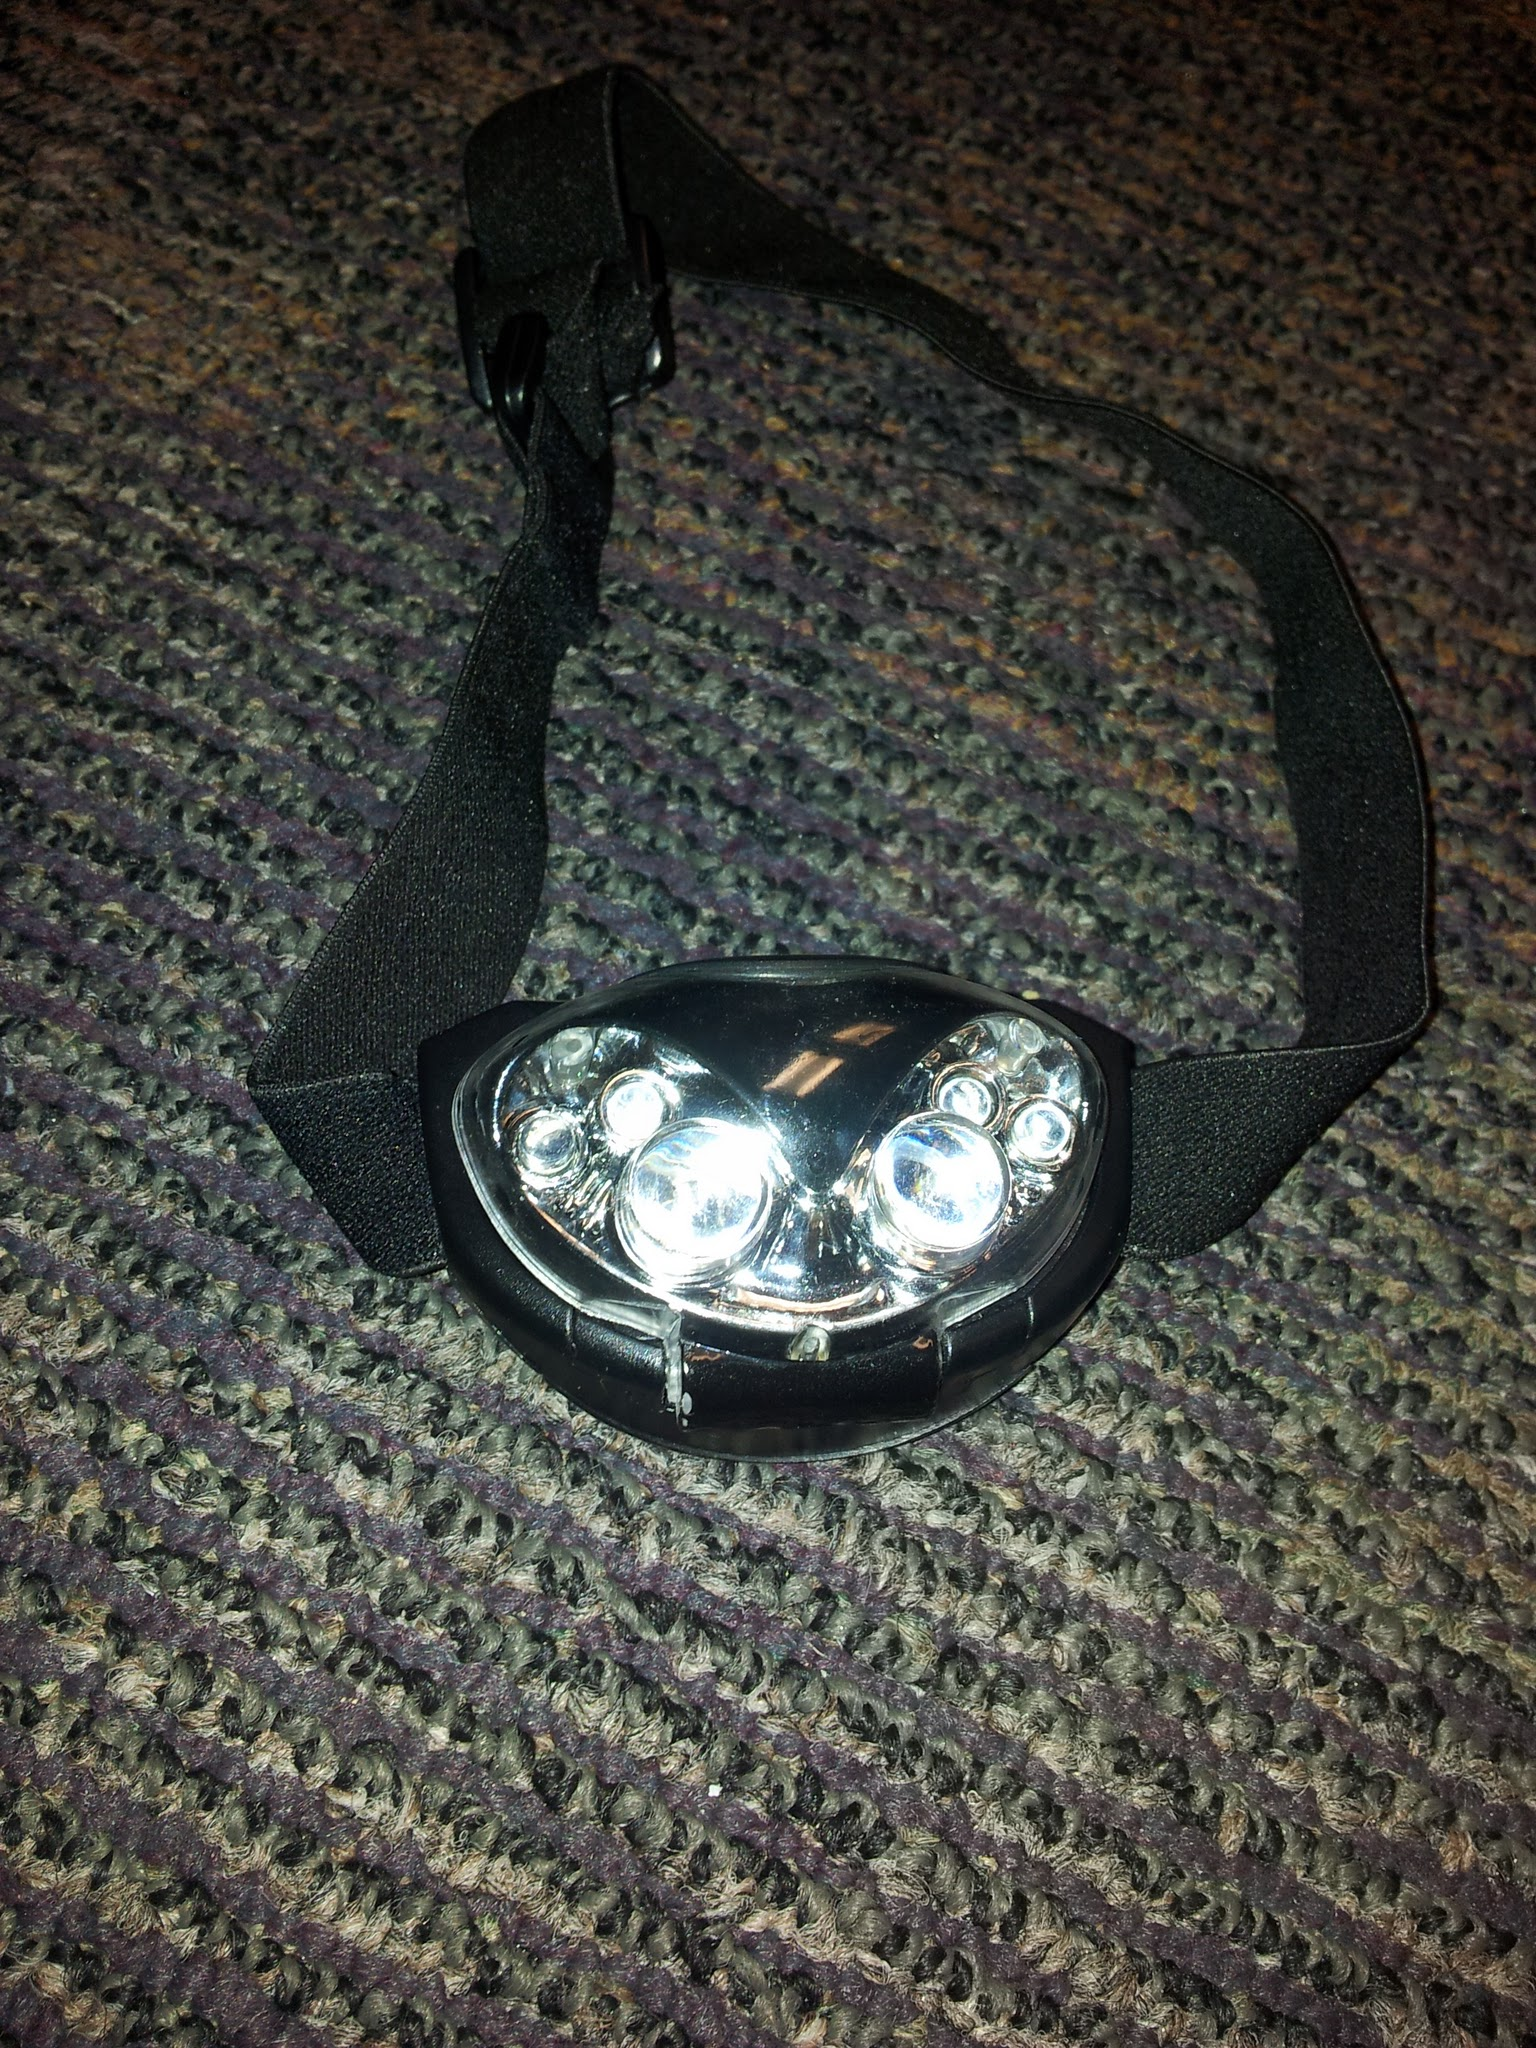
\includegraphics[scale=0.5]{headlamp}
\end{figure}

\section{The Lamp} The lamp is the main functional part of the headlamp. It is roughly 1/4 pounds
when loaded with it's 3 AAA battery power source. The lamp itself is split into two modules: the
bulb housing and the battery case. The two modules are joined by a hinge which allows the bulbs to
be aimed variably.

\subsection{Bulb housing}
\subsubsection{LED bulbs} The lamp has 6 main LED bulbs, 4 of the bulbs
are white and the remaining 2 are red. Of the 4 white LED's 2 of them have a radius of 0.5cm and are
located symmetrically opposite of each other 1cm away from the front center line of the lamp.  The
remaining 4 bulbs have a radius of 0.25cm and are aligned symmetrically opposite of each other
starting 2cm away from the front center line of the lamp. The bulb's furthest from the center line
are white, the inner bulbs are red.

\subsubsection{Casing} To protect the bulbs, a clear form fitting case covers the front of the lamp.
The case also acts to focus and intensify the light from the bulbs. The case consists of plastic and
is roughly 3mm thick.

\subsubsection{Power Toggle} Turning on the lamp is done with a plastic yellow power toggle located
on the top of the lamp directly above the casing and bulbs. The toggle is pressure sensitive.

\subsection{Battery Case} The majority of the headlamp is used to house the power supply. The supply
case is rectangular with rounded edges. It is 5cm across, 3cm wide, and 1.5cm deep. When in use the
back of the case is placed on to the wears forehead. To make this more comfortable there is a soft
black padding on the back 5cm by 3cm panel.

\section{The Strap} The strap serves the function of holding the headlamp to the users head. The
variable length strap is a maximum 2 feet long, and at it's minimum 1/2 foot long. It is made of an
elastic material that is black. The elasticity of the strap allows a strip of contracted material to
be stretched into a strip 3 times it's original length.

\section{Bulb settings}
The bulbs can be configured via the power toggle to emit three forms of light: Normal-White,
Bright-White, and Flashing-Red. These settings are achieved by powering some bulbs while not
powering others.

\subsection{Normal-White}
From the off state, toggling power once will place the headlamp into the Normal-White state.  This
setting power to the two main, 0.5cm radius, bulbs.

\subsection{Bright-White}
From the off state, toggling power twice will place the headlamp into the Bright-White state.  This
setting drives power to both the two main, 0.5cm radius, bulbs and the two outer white, 0.25cm radius, bulbs.

The headlamp emits the most light while in this state.

\subsection{Flashing-Red}
From the off state, toggling power three times will place the headlamp into the Flashing-Red state.
This setting drives power to the two inner, 0.5cm radius, red LED bulbs. While in this state the
bulbs will flash on and off at a frequency of 3 times per second. Each flash has a duration of
0.25 seconds.



% Just put plain text here
% render with 'pdflatex <file.tex>'
something in section

\end{document}
